\documentclass{ctexart}
\usepackage{graphicx}
\usepackage{ctex}
\usepackage{listings}

\usepackage{tikz}
\usetikzlibrary{arrows, decorations.pathmorphing, backgrounds, positioning, fit, petri, automata}
\definecolor{yellow1}{rgb}{1,0.8,0.2}




\author{xzx}
\title{assignment2我的答案}


\begin{document}
\maketitle
\setcounter{page}{0}
\thispagestyle{empty}
\newpage

\begin{flushleft}

\section{Q1: Fully-connected Neural Network}

\subsection{/cs231n/layers.py}

\subsubsection{affine\_forward \& affine\_backward}
\paragraph{affine\_forward}没什么好说的,就是正常的相乘就完了。\\
\paragraph{affine\_backward}需要注意的地方是再对dout求和的时候,参数keepdims=True很有用。假设
dout是(N,M)的矩阵,
\begin{lstlisting}[language=python]
  np.sum(dout,axis=0)#返回一个(M,)的矩阵
  np.sum(dout,axis=0,keepdims=True)#返回一个(1,M)的矩阵
\end{lstlisting}


\subsubsection{/cs231n/classifiers/fc\_net/py}
\paragraph{TwoLayerNet}
与assignment1不同的是,这里的两层网络加上了一个relu层。在做作业的时候,开始忘掉了relu层,
导致不论怎么调hyper parameter训练集上面的accuracy最高只能到达43\%。因为affine层是线性
层,线性层不论怎么叠加的效果都是线性层,所以没有relu的情况下准确率很难提高

\subsection{update rules}
课程中介绍了几种主流的更新W的方法。想象当前所在的位置是山谷中随机的一个位置,目标是走到山谷
的底部。\\
最简单的就是SGD,每次按照偏导数的方向(下山的方向)走一小步,直到走到结束条件为止。\\
第二种方法是Momentum。假如一个小球从山谷的某个地方向下滚,这个小球会有一个当前速度,还有一
个加速度的方向,它下一步的速度方向应当是由当前速度和当前加速度一起决定的。所以再计算的时候
要记录下当前的速度,把偏导数的方向当做加速度的方向。
\begin{lstlisting}[language=python]
  v = mu*v - learning_rate*dx
  x += v
\end{lstlisting}
这里可以把mu认为是在向下滚动时候碰到的摩擦力
第三种方法是AdaGrad。在视频中可以看到SGD的一个缺点是它会沿着偏导数较大的方向走很远,但是偏导数
较小的方向走的步伐会很小,这样在向谷底走的时候,会产生很大的震荡。
\begin{lstlisting}[language=python]
  #Adagrad update
  cache += dx**2
  x += - learning_rate * dx / (np.sqrt(cache) + 1e-7)
\end{lstlisting}
cache的作用就是不让更新的步伐沿着偏导数较大的方向走太远。加上$10^{-7}$仅仅是为了防止除数
为零。当更新次数很多的时候,cache会逐渐变得很大,更新的步长就会逐渐变小。\\
在AdaGrad的基础上,Hinton提出了RMSProp。思路是差不多的,仅仅是cache变化了一下。\\
将AdaGrad和Momentum合在一起,就是Adam。


\section{Q2: Batch Normalization}

在训练神经网络的时候,会出现一个问题,在较深层的神经元,信号数值的分布很难看。这就导致了训练
出来的神经网络对learning\_rate非常敏感。
Batch Normalization的思路就是在每一层加上一个Batch\_Norm层,保证每层神经元得到的数据都
符合正态分布。这样做的结果是会降低神经网络的表现力,所以要让Batch Norm学习shift和scale,
shift是正太分布的中心,scale是方差(代码里面是gamma和beta)。

\begin{tikzpicture}[->,>=stealth',shorten >=1pt,auto,node distance=2.8cm,
                    semithick]
  \tikzstyle{every state}=[fill=yellow1,draw=none,text=black]
  \tikzstyle{divbelow}=[below,text=gray]
  \tikzstyle{divabove}=[above,text=gray]
  \node[state]  (X)         at (-5,6) {$X$};
  \node[state]  (minus)     at (-3,6) {$-$};
  \node[state]  (star1)     at (4,6) {$*$};
  \node[state]  (star2)     at (6,6) {$*$};
  \node[state]  (plus)      at (8,6) {$+$};
  \node[state]  (mu)        at (-4,4) {$\mu$};
  \node[state]  (sqr)       at (-2,4) {$\^2$};
  \node[state]  (var)       at (0,4) {$\frac{1}{n}\sum$};
  \node[state]  (sqrtvar)   at (2,4) {$sqrt$};
  \node[state]  (ivar)      at (4,4) {$\frac{1}{t}$};
  \node[state]  (gamma)     at (-5,2) {$\gamma$};
  \node[state]  (beta)      at (-5,0) {$\beta$};
  \node[state]  (out)       at (10,6) {out};

  \path (X)       edge            node {$x$}        (minus)
                  edge            node {$x$}        (mu)
        (mu)      edge            node {$\mu$}      (minus)
        (minus)   edge            node {$x-\mu$}    (star1)
                  edge            node {$x-\mu$}    (sqr)
        (sqr)     edge            node {$(x-\mu)^2$}(var)
        (var)     edge            node {$var$}      (sqrtvar)
        (sqrtvar) edge            node {$sqrtvar$}  (ivar)
        (ivar)    edge            node {$ivar$}     (star1)
        (star1)   edge            node {$\hat{x}$}  (star2)
        (star2)   edge            node {}           (plus)
        (plus)    edge            node {}           (out);
  \draw[->] (gamma) to[out=0,in=-90]  node {$\gamma$}   (star2);
  \draw[->] (beta)  to[out=0,in=-90]  node {$\beta$}    (plus);

  \node[divbelow] (dstar1)     at (5,6)      {$\partial{\hat{x}}$};
  \node[divbelow] (dminus1)    at (0,6)      {$\partial{(x-\mu)_1}$};
  \node[divbelow] (dx)         at (-4,6)     {$\partial{x_1}$};
  \node[divbelow] (dout)       at (9,6)      {$\partial{out}$};
  \node[divbelow] (dout1)      at (7,6)      {$\partial{out}$};
  \node[divbelow] (divar)      at (4.5,5)    {$\partial{ivar}$};
  \node[divabove] (dsqrtvar)   at (3,3)      {$\partial{sqrtvar}$};
  \node[divabove] (dvar)       at (1,3)      {$\partial{var}$};
  \node[divabove] (dsqr)       at (-1,3)     {$\partial{(x-\mu)^2}$};
  \node[divbelow] (dminus2)    at (-2.5,5.3) {$\partial{(x-\mu)_2}$};
  \node[divbelow] (dmu)        at (-3.5,5)   {$\partial{\mu}$};
  \node[divbelow] (dx2)        at (-4.8,5)   {$\partial{x_2}$};
\end{tikzpicture}
这个图差不多是整个作业里面最复杂的一个反向传播的图了。借鉴了网上的一个博客,具体
地址忘记了。。。\\
$\beta = \sum{\partial out}$这个应该不难理解。\\
而$\partial out$仅仅是经过了一个加法运算,所以再加号左边仍然不变.\\
另外在前面,第一个节点X跟减号的节点有分叉。对于分叉的节点,偏导数就把各个分支的
偏导数加起来。
剩下的就按照反向传播往前传就好了。

\section{Q4: ConvNet on CIFAR-10}
\subsection{Spatial Batch Normalization}
在卷积网络里的Batch Normalization与普通的Normalization不太一样。如
\ref{fig:spatial_batch_norm}所示。
\begin{figure}[h]
  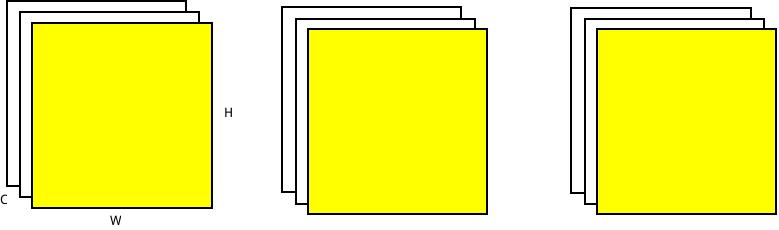
\includegraphics[width=5in]{./assignment1_pic/spatial_batchnorm.jpg}
  \caption{spatial\_batch\_normalization}
  \label{fig:spatial_batch_norm}
\end{figure}
标准化的过程是要将黄色的地方求均值与方差。所以要用到python中的一个函数来交换数组的
维度。交换完成以后就万事大吉了。


\end{flushleft}
\end{document}
